\documentclass[usenames,dvipsnames]{article}
\usepackage{amsmath}
\usepackage{amsfonts}
\usepackage[letterpaper, total={6in, 8in}]{geometry}
\usepackage{color}
\usepackage{xcolor}
\usepackage{graphicx}
\usepackage{booktabs}
\newcommand{\todo}[1]{\textcolor{red}{#1}}

\providecommand{\response}[1]{
\noindent
\noindent\colorbox{gray!20}{
\parbox{\textwidth}{
\setlength{\parskip}{.1in}
\setlength{\parindent}{.1in}
#1}
}
}


\title{\LARGE Real-Time Certified Probabilistic Pedestrian Forecasting \\ \textbf{Author's Response} }

\author{Henry O. Jacobs, Owen Hughes, \\ Matt Johnson-Roberson, and Ram Vasudevan }

\begin{document}
\maketitle

%\todo{More formal version of: We would like to thank the reviewers for their comments. The feedback is very helpful, and we have attempted to address everything.}

We would like to begin by thanking the reviewers and the editor for their careful reading and review of our paper.
The comments provided were incredibly helpful and insightful, and have strengthened the paper considerably.
Based on the recommendations of the reviewers and the editor, we have made several modifications to the paper.
%The changes made are presented below as a highlighted manuscript that indicates additions in green and removals in red.
The changes made are summarized in detail below and a highlighted manuscript is attached that indicates additions in red.
% See the response to reviewers for a detailed breakdown of the changes made.

\section*{Reviewer 1}
\begin{enumerate}

\begin{item}
\textbf{This paper presents a novel real-time probabilistic forecasting method
for pedestrian trajectories via observing the historical trajectories
in a particular scene. The problem is well motivated, formulated and
handled. The reported experimental evaluations show pivotal improvement
against the current state-of-the-art.}

Thank you for the positive assessment.
\end{item}

\begin{item}
\textbf{With the current form of the results it is hard to compare the
improvements in terms of accuracy gained. This can be overcome by
including results such as physical distance between predicted paths and
ground truth observations. Such matrices are provided in the baseline
models [7, 9, 13] with accuracy values in meters. }

Thank you for noticing the difficulty in comparing the improvements. We calculated the MHD from each point in the trajectory to sampled points from each distribution which is summarized in Figure \ref{MHD} below. 

We feel that both plots add something to the analysis, so we've included the following passage to justify both our metrics.

\response{ In our analysis we sought a metric that measured the similarity between the predictor and the ground truth as well as the ``safety'' of the prediction. We used the area under the curve of the ROC curve as our measure of this. The ROC curve plots the rate of false positive detections against the probability of detecting a pedestrian, or in essence the quality of the detection versus the safety. The area under this curve is a standard measure of the quality of a predictor. Figure \ref{AUC} shows the analysis of the AUC of each algorithm versus time. In addition, we used the Modified Hausdorff Distance (MHD) from the ground truth trajectory to a sample from the predictions at each time in order to provide a geometric measure of how accurate the predictions are. Figure \ref{MHD} shows MHD plotted against time.}

\end{item}
\begin{figure}
	\centering
	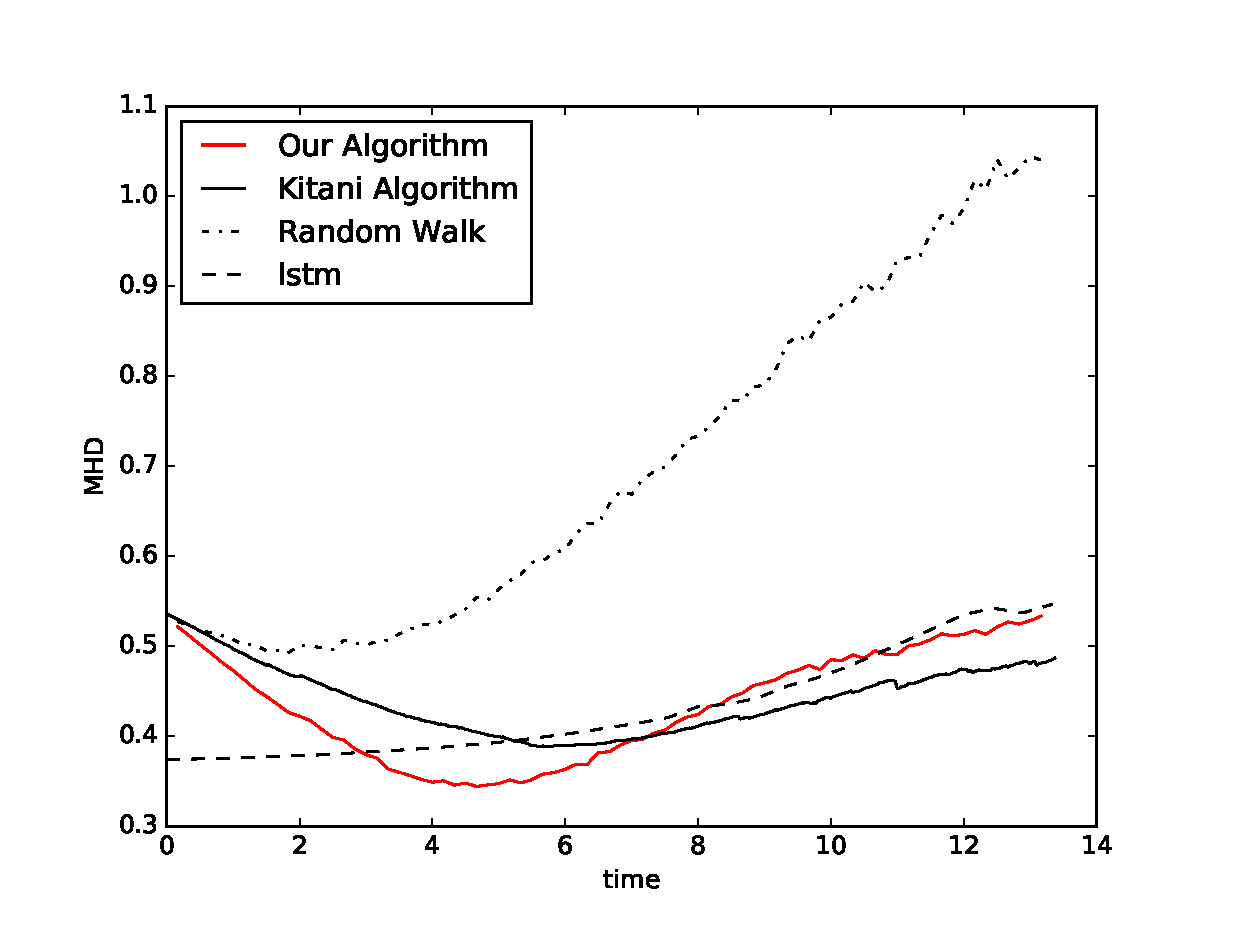
\includegraphics[width=0.6\textwidth]{paper/figures/mhd_results.eps}
	\caption{A comparison of the Modified Hausdorff Distance from the ground truth of the pedestrian to a 1000 point sample from each distribution. The method from [13] does very well at short time scales due to its confidence, but we outperform all other methods at intermediate times. At long timescales the MHD to the trajectory of most algorithms converges. Our method increases positional uncertainty with time, and so [7] outperforms us because they know the end point and we do not, and [13] places too much significance on the positions of other pedestrians at large time scales.}
	\label{MHD}
\end{figure}

\begin{figure}
	\centering
	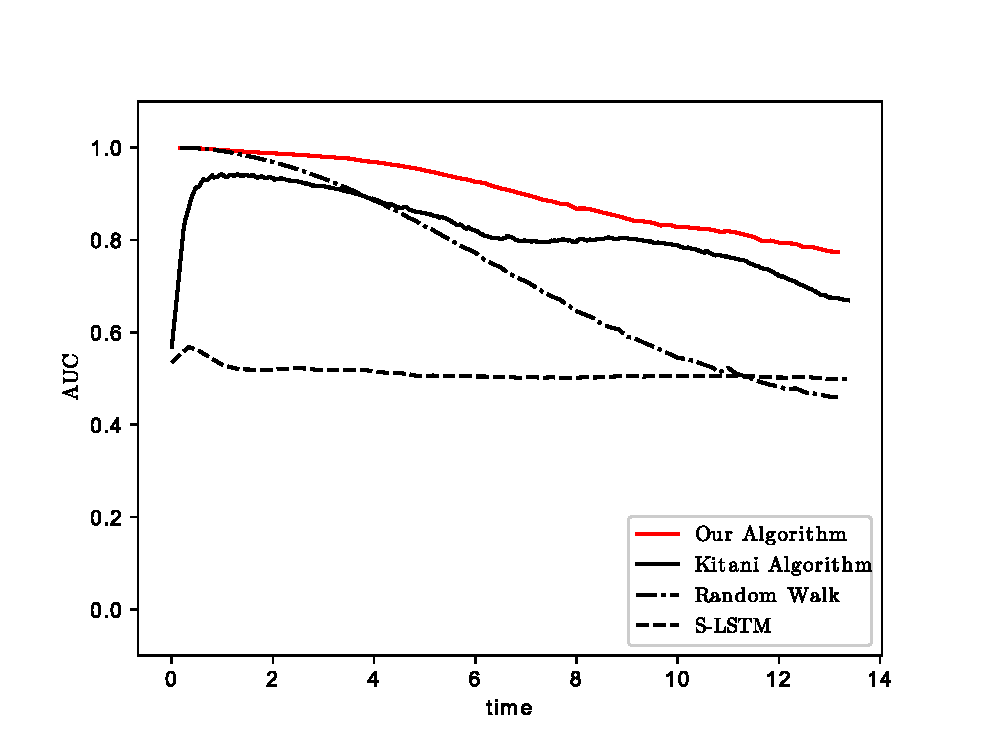
\includegraphics[width=0.6\textwidth]{paper/figures/the_results.eps}
	\caption{A comparison of the AUC of the various algorithms. Note that the initial dip in the performance of [7] is due to their confidence in their initial estimate. We sampled the S-LSTM model 100 times in order to give them the best chance in this analysis, but their confidence combined with the over-reliance on social forces at moderate-to-large lowered their performance.}
	\label{AUC}
\end{figure}

\begin{item}
\textbf{How the model can incorporate the interactions among pedestrians (i.e
group motion) and the influences from neighbouring pedestrians (for
instances such as collision avoidance)?}
\end{item}
Thank you for this insightful question. Social forces are a natural avenue for future work, and so we included the following paragraph in the paper.

\response{Though including social forces into the model is out of the scope of this paper, incorporation could begin as follows.  In the current motion model with a single vector field, the acceleration of the $i$th agent is given by $\ddot{x}_i = s^2 DX(x_i) \cdot X(x_i)$.  Incorporating a social force $F_{i}$ acting on the $i$th can be done by instead asserting $\ddot{x}_i = s^2 DX(x) \cdot X(x) + F_i$.  Usually $F_{i} = \sum_{j} \nabla U( x_j - x_i)$ where $U$ is an interaction potential \todo{[Helbing and Molnar]}.}


\begin{item}
\textbf{Presentation and organisation
The motivation behind choosing start/end points based clustering is not
clear. Does clustering based on start/end points help to identify
different motion models? Isn't it better to cluster considering the
entire trajectory? }
\end{item}
This is a relevant question, thank you. As stated in Morris and Trivedi (below), our choice of clustering technique is not nearly as important as the chosen distance metric. Our success with distance functions that took a whole trajectory was limited on the data we tested, particularly when compared against our method. We have several hypotheses as to why this is true.  For one, the spatial scale of the data we test against showcases important features (e.g. curb cuts and storefronts), which lead to clustered start points and end points. Similarly, we tested against high quality data in which trajectories with irreconcilable occlusions were rare and thus could be omitted. See the comment below for the text we added to the paper.



\begin{item}
\textbf{Do you cluster different scenes provided in campus dataset [13] (i.e
Valley, Fangron) separately or all together? When motion models are
learnt, are they learnt in scene specific manner or altogether?}
\end{item}
Thank you for noticing that this is unclear. Our algorithm trains on each scene independently, so clustering, vector field learning, and learning the potential functions are all done for each Valley, Fangron, etc. We've added the following text to the paper:

\response{We did a 2-fold cross validation by using 20\% of the data for testing and the remainder for training within each scene. We learned separate collections of vector fields and model parameters for each fold on all of the four scenes on which we tested.}


\begin{item}
\textbf{The motivation behind choosing the affinity propagation clustering
algorithm is not clearly stated. 
What is the distance measure used (i.e Euclidian, \"{O}) ? Not specifying
such information makes reproduction of this work not feasible. }

This was an oversight on our part, thank you for noticing it. The distance used is actually a custom distance function on $\mathbb{R}^4$, which disregards the involution $(x_1, x_2, x_3, x_4) \to (x_3, x_4, x_1, x_2)$, and so doesn't care about parity of trajectories. We have included the following clarification:

\response{We then cluster in $\mathbb{R}^4$ using Affinity Propagation[17] and a custom distance measure defined by $d((x_1, x_2, x_3, x_4),\mathbf{y}) : \mathbb{R}^4 \times \mathbb{R}^4 \to \mathbb{R} = \min \left\{ d_e((x_1, x_2, x_3, x_4), \mathbf{y}), d_e((x_3, x_4, x_1, x_2), \mathbf{y}) \right\}$, for the euclidean distance $d_e$. This function measures the distance between the endpoints irrespective of their ordering. The scale of the datasets we tested on had large enough spatial scale that clustering based on endpoints captured people moving from destination to destination, e.g. from a storefront to the sidewalk at the edge of a scene. On our data, other distance measures from \todo{[Morris and Trivedi]} and \todo{[Lee 2007]} didn't identify coherent motion models. This is partly due to the fact that oftentimes pedestrians would take slightly different routes to get to their destination, but the cumulative effect on the distance measures is enough to hinder the clustering. }
	
\end{item}

\begin{item}
\textbf{Adequacy of Citation
I believe literature review section can be improved using a sub section
on social force models, which is extensively applied for pedestrian
trajectory forecasting. 
Helbing and Molnar, 1995; Koppula and Saxena, 2013; Pellegrini et al.,
2010; Yamaguchi et al., 2011; Xu et al., 2012; Wang et al. 2008;
Hospedales et al. 2009; Emonet et al. 2011; Yi et al. 2015.}
\end{item}

We agree that this adds to the paper, thank you for the suggestion. We added a section to our literature to reflect the relevant work.

	\response{On the other hand, authors have approached pedestrian forecasting by deriving their motion model from interactions between pedestrians. Early work by [helbig] and [Xu] describe pedestrians interactions using physically motivated tools. Several models [yamaguchi, yi, pellegrini you’ll never] derive their motion models from [helbing] which incorporates collision avoidance through an interaction potential which repels pedestrians from each other, leading to forms of Linear Trajectory Avoidance (LTA). However LTA suffers from not planning for other pedestrian’s positions at future times. [emonet], [hospedales], and [wang: unsupervised] all take optical flow as input. [wang] and [emonet] both use variants of Hierarchical Dirichlet Processes on discretized optical flow to determine temporal motifs (i.e. classes of motion within the scene), where [hospedales] substitutes a Markov model. These models are not agent based, and the lack of an explicit motion model limits their predictive power in situations where we know more about the data. [koppula and saxena] predict trajectories by introducing and sampling Anticipatory Temporal Conditional Random Fields which incorporate human affordances relating to human objectives within the scene. [Tay], [Wang jw], and [Trautman] create agent-based models based on Gaussian Processes, though they suffer issues when trained on discretized trajectories. [alahi] uses Long Short-Term Memory to learn pedestrian motion models without making implicit (as in the case of CRFs) or explicit (in the case of social forces) assumptions about the manner in which agents will interact. [alahi] outperformed LTA, and social forcing based on [yamaguchi]  and IGP from [trautman]. Along with its quick run time, this motivated our decision to test our algorithm against it.  }

\begin{item}
\textbf{Furthermore a comprehensive review on trajectory clustering algorithms
is required. This should be used to motivate the reason of choosing
affinity propagation algorithm in section 4. 
Morris and Trivedi 2009; Giannotti et al. 2007; Lee et al. 2007;
Ester et al. 1996 }

Thank you for this suggestion and for the list of relevant titles. We included a note about different algorithms as well as a justification for why we chose our metric. The note can be seen in point 6 above.

\end{item}
\end{enumerate}


\section*{Reviewer 2}
\begin{enumerate}
\begin{item}
\textbf{Keep the good work going. Interesting approach.}
\end{item}

Thank you for the kind comments.
\begin{item}
\textbf{
Need to be clearer and
dive a little bit deeper into the technical approach. }
Thank you for this criticism. We hope we adequately addressed it by strengthening the description of our method for learning the motion model, as well as quantifying the way that we tested our data. We also changed the language below to better reflect that the specific implementation we chose is an example of how to use the larger framework.

\response{Given the model established in the previous section, we describe an implementation to showcase one way the model can be applied to observational data.}
\end{item}
\begin{item}
\textbf{
Need to use and apply more deep learning approaches such as social LSTM
or other machine methods.}
Thank you for the suggestion. We hope that we have addressed it by including a review of literature of social force models, including S-LSTM, as well as a section on how social factors can be integrated into our model. In addition, we compared against S-LSTM in addition to [7] from the paper. Thefigures drawing the predictions of the S-LSTM model are ommitted from the paper because like many of the agents, the S-LSTM predictions quickly exit the bounds of the scene, and so the visualization is identically zero. We changed the subtitle of the figure to reflect this, which is shown below.

\response{An illustration of the predictions generated by the various algorithms. In this figure, the dot is the start point of the test trajectory, the diamond is the position at time t, and the X is the end of the trajectory. The likelihood of detection is depicted using the virdis color palette. Notice that the Random Walk is imprecise, while the predictions generated by the algorithm in [7] suffer from the inability of their motion model to adequately match the speed of the agent. The algorithm from [13] quickly passes beyond the boundaries of the scene, so the plots are ommitted here.
}
\response{An illustration of the predictions generated by the various algorithms. In this figure, the dot is the start point of the test trajectory, the diamond is the position at time t, and the X is the end of the trajectory. The likelihood of detection is depicted using the virdis color palette. Notice that the Random Walk is imprecise, while the predictions generated by the algorithm in [7] are unable to match the speed of the agent and choose the wrong direction to follow the agent around the circle. The algorithm in [13] passes beyond the boundaries of the scene, and so the plots are ommitted here.}

\end{item}

\end{enumerate}

\section*{Reviewer 5}
\begin{enumerate}
\begin{item}
\textbf{
It would be more interesting if the authors show whether
the prediction algorithm would transfer the learned "knowledge" of
forecasting in novel scenes.}
Thank you for your comment. As it is, this is a shortcoming of our model, but we see it as an immediate avenue for future work. As can be read below, the environmental decomposition that the segmentation algorithm in [12] returns as well as an analogue of the methods [11] proposes for characterizing and transferring our vector fields from one scene to another.

\response{As future work, we propose using scene segmentation from [12], as well as the semantic context descriptors and routing scores from [11] to show how vector fields can be transferred to novel scenes. It appears that the low-order parameterization of our model, and unit-length vector field assumption make it particularly amenable to the methods developed in [11].}


\end{item}
\begin{item}
\textbf{
More statistically result is expected
rather than analyzing "four different scenes", and comparing run-time
by "averaged across several agents and scenes" (how many?).}

Thank you for noticing this. We've clarified the papers in the passages listed below to clarify the list of scenes we ran in comparison, and how many agents total were run. We clarified that the set of agents used to evaluate were the same that were used to determine run times. Note that we attempted to compare on all of the scenes in the Stanford Drone Dataset, but the difficulty in getting the other models to converge in a reasonable amount of time prevented us from doing so.

\response{ Our analysis was conducted on the Coupa, Bookstore, Death Circle, and Gates scenes from the dataset from [13], with a total of 142 trajectories analyzed.}

\response{The run time per frame for each algorithm was generated using the mean run time for 400 frames, averaged across all of the data used in the quality analysis.}
\end{item}

\begin{item}
\textbf{
Besides, it is better to explain the meaning of ROC and AUC in section IV.}

This is a necessary clarification, thank you for the suggestion. We have included a description of ROC and AUC, as well as a justification for why we chose to evaluate the methods using this criterion. You can read the text that we added to address this in the second point made by Reviewer 1.

\end{item}
\end{enumerate}

% \section*{Associate Editor?}
% \begin{enumerate}
% \begin{item}
% \textbf{The manuscript presents an interesting approach toward pedestrian
% forecasting which is quite different than current approaches.}  
% \end{item}
% \begin{item}
% \textbf{The
% presentation could be improved by providing more concrete performance
% measures and comparison with more state-of-the-art.For example newer
% models that utilize social interactions.  Please see the reviewer
% comments for more detailed recommendations.}
% Thank you for the suggestions, we feel that they have added to the quality of the paper. As stated in the individual responses to reviewers, we tested using a variant of the MHD method used in [7], and found that while we still outperformed [7] and [13] in the intermediate time scales, it didn't capture our desire to test for safety as well as proximity to ground truth as well as the AUC of the ROC curves. The plot of measured MHD is included \todo{(?)}.

% The addition of a comparison to social interaction models was very valuable, and we thank you for the suggestion. We have included a section in our literature review on these models, as well as a comparison in section IV to the S-LSTM model from [13].

% \end{item}
% \end{enumerate}


\end{document}